Section \ref{sec:mod_desc} gives descriptions of each model and provides both Ordinary Differential Equations and the constitutive functions that describe each model's fluxes. These constitutive functions and any relevant constraints are implemented in MARRMoT as individual \emph{flux files}. Each \emph{flux file} contains computer code that combines the constitutive function and constraints (if needed). \emph{Flux files} are located in the folder ''./MARRMoT/Models/Flux files/''. The User Manual contains details on understanding, modifying and creating new \emph{flux files}. Table \ref{tab:sm2_1} shows a complete overview of fluxes currently implemented in MARRMoT.

% Place a caption
\vfill{}
\captionof{table}[Computational implementation of constitutive flux equations]{Equations from model descriptions and their implementation in MARRMoT (Table starts on following page) \label{tab:sm2_1}}


% BIIIIIIG table
%\afterpage{\clearpage}

\clearpage
\KOMAoptions{paper=A3,paper=landscape,pagesize}
\recalctypearea



%\begin{landscape}
%\pagestyle{empty} 	% remove page numbers
%\centering
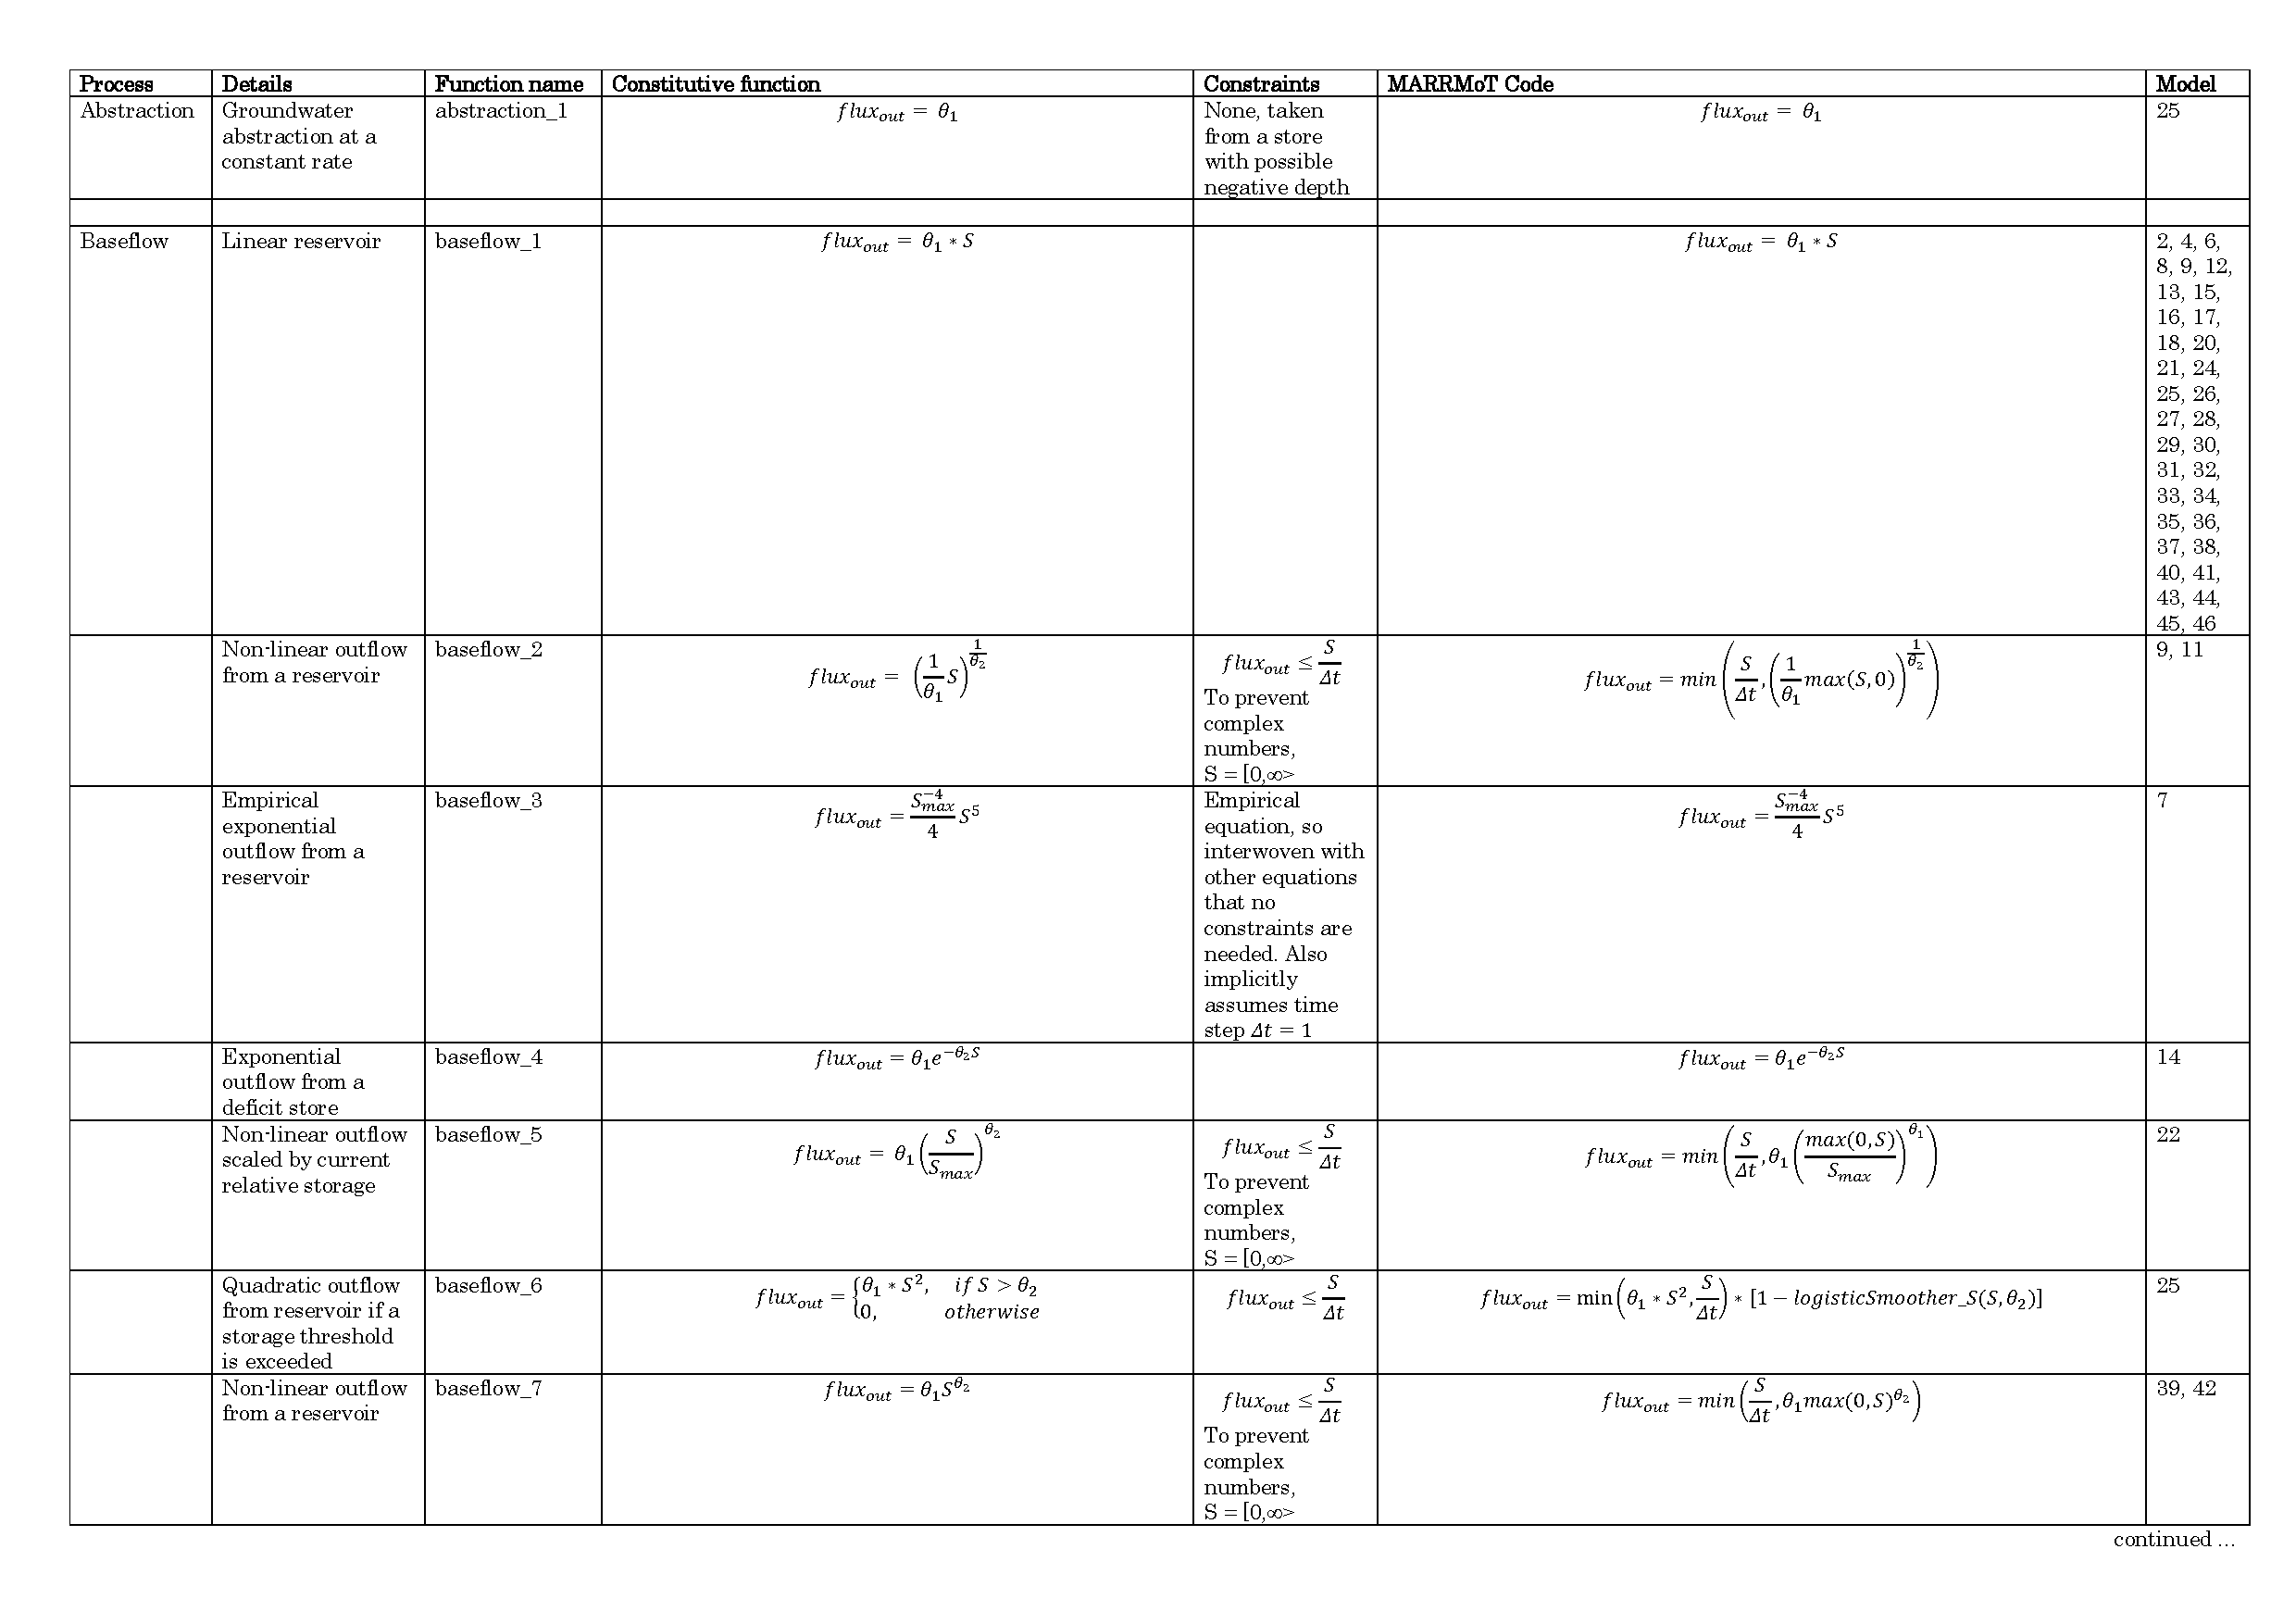
\includepdf[pages=-,pagecommand={\thispagestyle{styleLandscapeA3}}]{sm2_fluxes.pdf}
%\end{landscape}

% 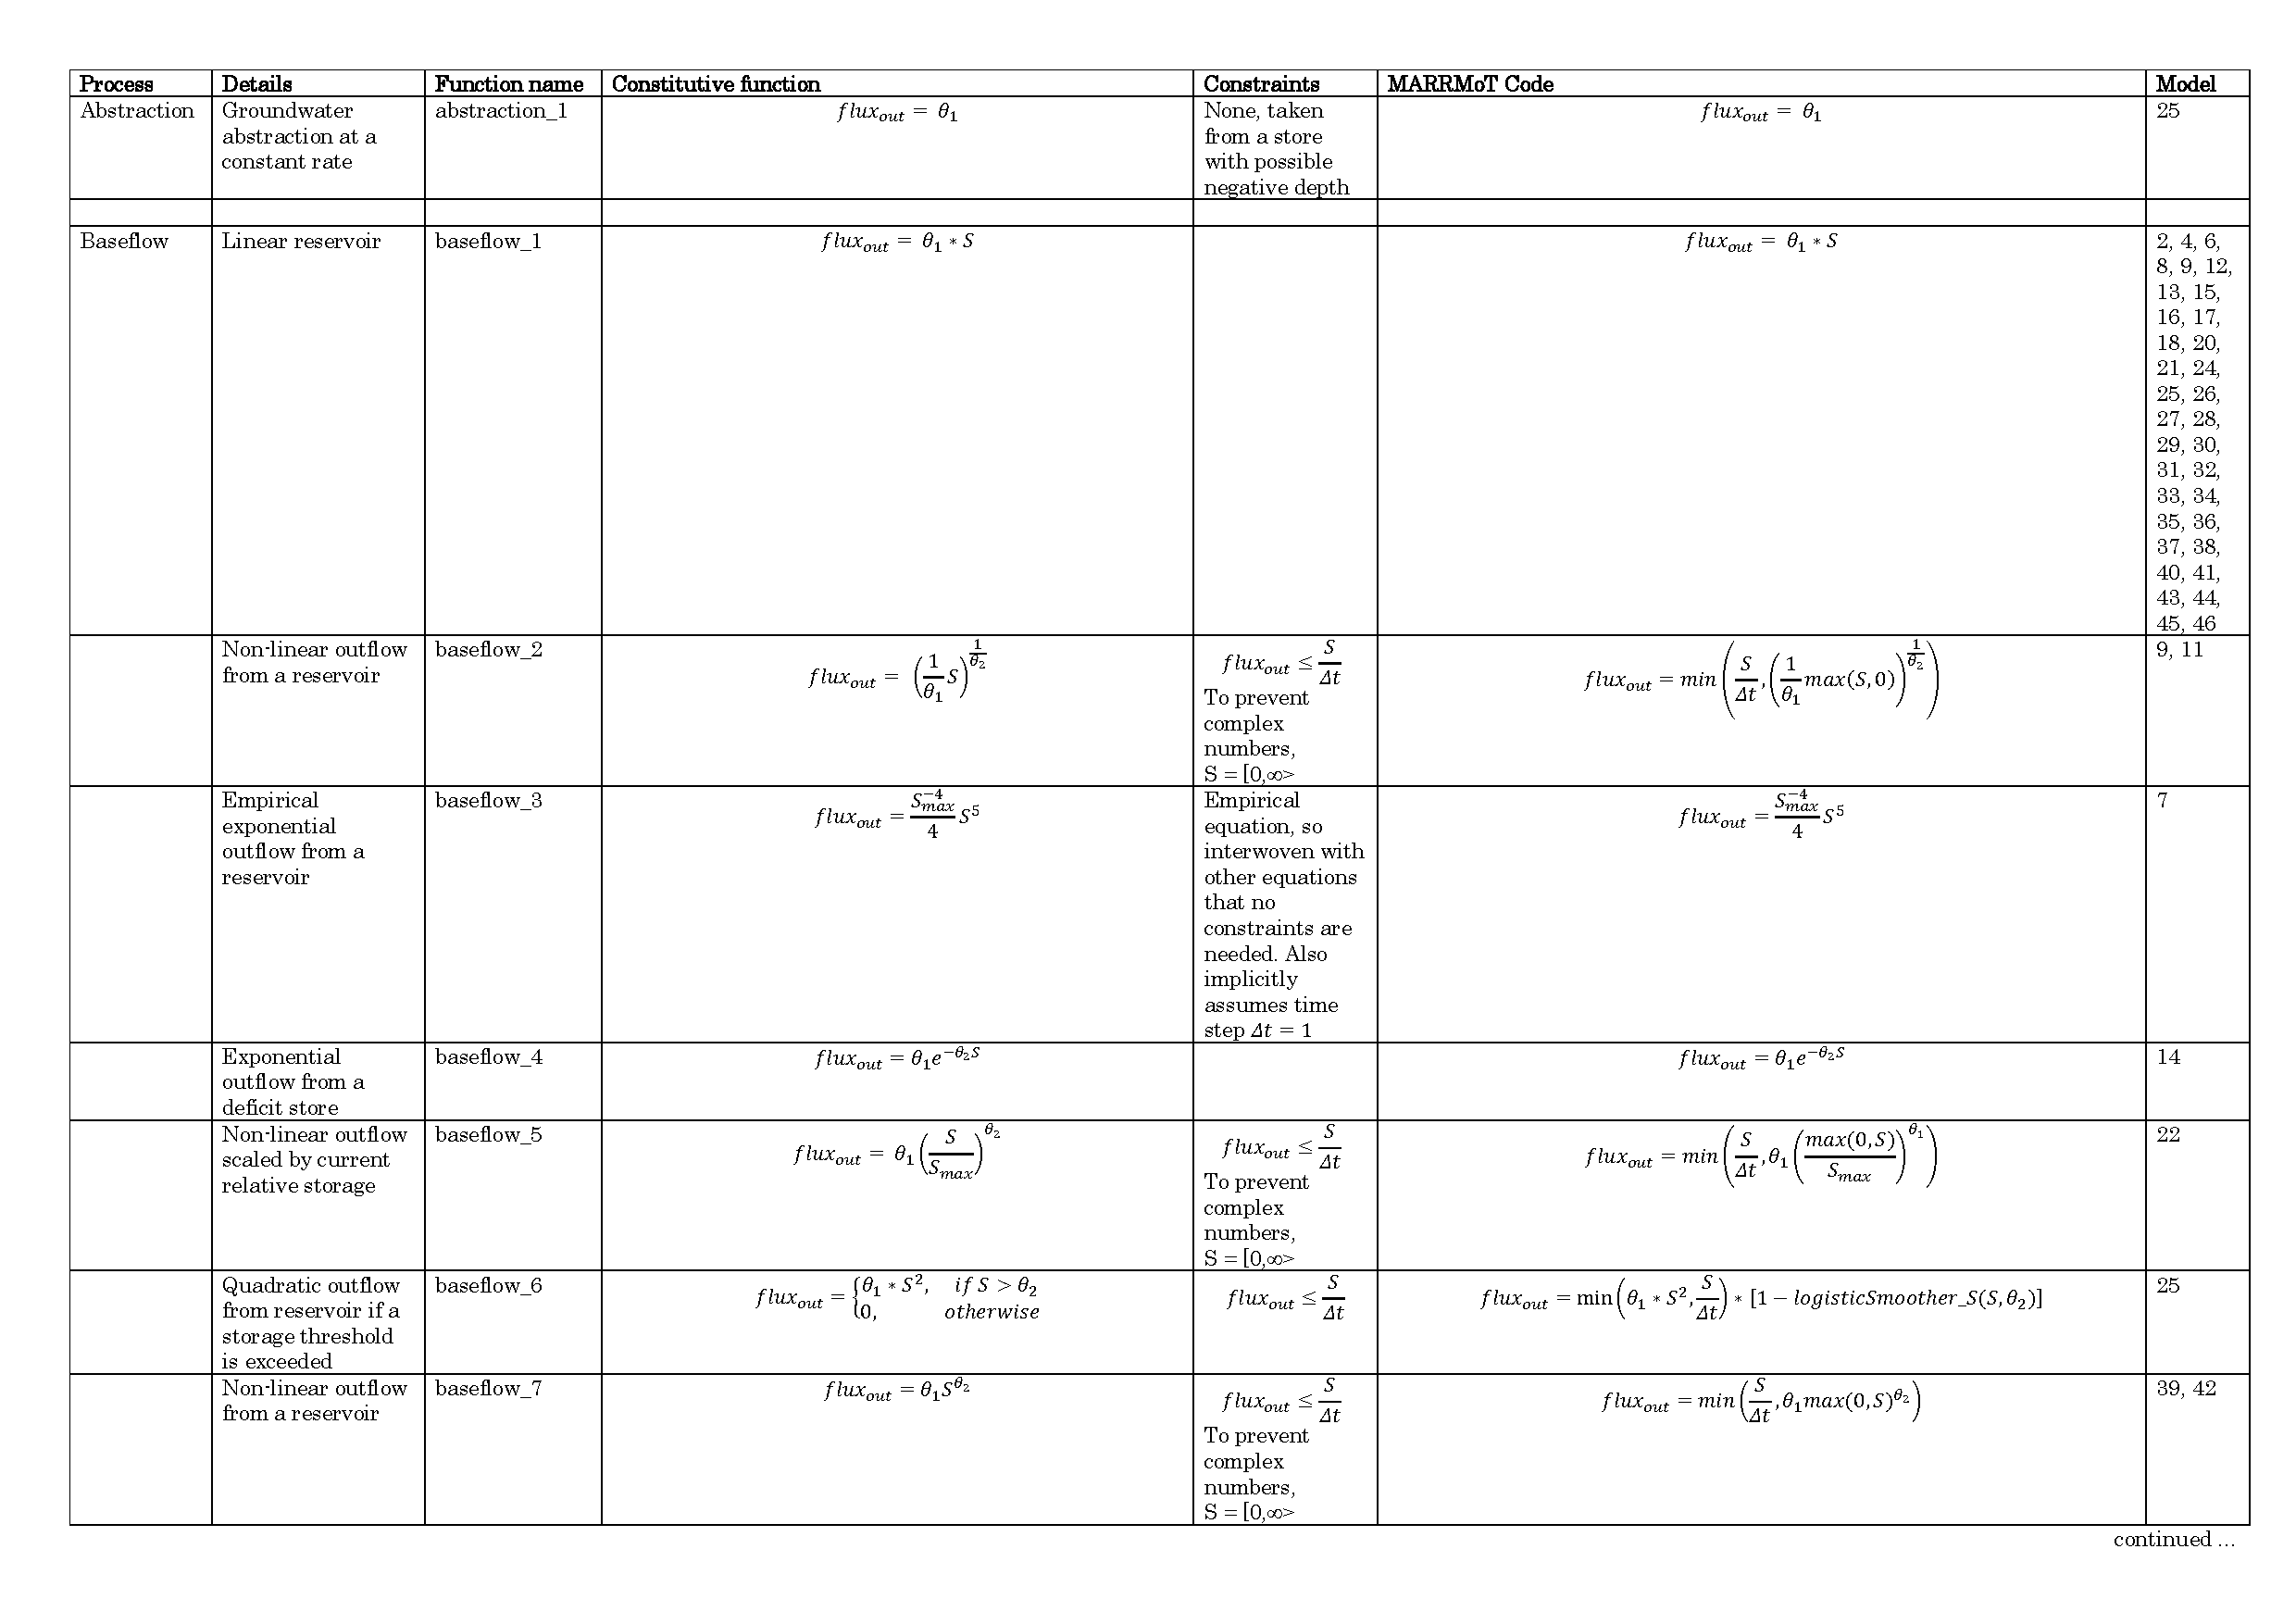
\includepdf[pages=-,landscape,pagecommand={\thispagestyle{styleLandscape}}]{sm2_fluxes.pdf}


\clearpage
\KOMAoptions{paper=A4,paper=portrait,pagesize}
\recalctypearea























